\documentclass{article}
\usepackage[utf8]{inputenc}
\usepackage[T1]{fontenc}
\usepackage{graphicx}
\usepackage{amsmath, amssymb}
\usepackage{xcolor}
\usepackage{tikz}
\usepackage{enumitem}
\usepackage{lipsum}
\usetikzlibrary{fit}
\usepackage{mathtools}
\usepackage{hyperref} 
\usepackage{subfig}
\usepackage{polynom}
\usepackage{pgfplots}
\usepackage{soul}
\usepackage{framed}
\usepackage[most]{tcolorbox}
% Define colors
\definecolor{lessoncolor}{RGB}{74, 144, 226}
\definecolor{examplecolor}{RGB}{92, 184, 92}
\definecolor{notecolor}{RGB}{255, 179, 102}

% for the angle arc
\usetikzlibrary{angles,quotes}

% for arrow tips
\usetikzlibrary{arrows.meta}

\begin{document}

\begin{titlepage}
    \centering
    \vspace*{2cm}
    {\LARGE \textcolor{lessoncolor}{Advanced Functions}}\par
    \vspace{1cm}
    {\large Kensukeken}\par
    \vspace{2cm}
    {\large April 11th, 2024}\par
    \vspace{3cm}
\end{titlepage}
\tableofcontents
\newpage
\section{Unit 4}
\subsection{Radian Measure}
If you draw a circle with center $O$ and radius $r$, and you draw two radii $OA$ and $OB$, then you can define length $AB$ as an arc $a$ and angle $AOB$ as $\theta$.
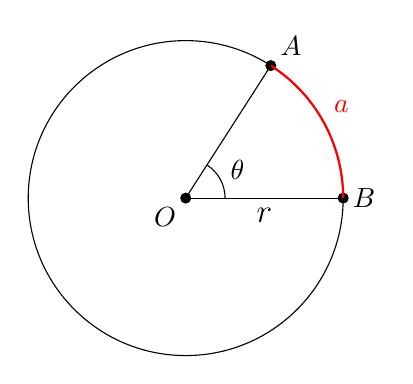
\begin{tikzpicture}
    % Define radius
    \def\radius{2cm}

    % Draw circle
    \draw (0,0) circle (\radius);
    
    % Define center, points A and B
    \coordinate[label=below left:$O$] (O) at (0,0);
    \coordinate[label=above right:$A$] (A) at (57.2958:\radius);
    \coordinate[label=right:$B$] (B) at (0:\radius);
    
    % Draw points
    \foreach \point in {O, A, B}
        \fill (\point) circle (2pt);
    
    % Draw arc AB
    \draw[thick, red] (A) arc (57.2958:0:\radius) node[midway, above right] {$a$};

    \draw (B)--(O) node[midway, below, font=\large] {$r$};

    \draw (O)--(A);
    
    % Draw and label angle AOB with theta
    \pic[draw, "$\theta$", angle eccentricity=1.5] {angle = B--O--A};
\end{tikzpicture}

The Radian Measure is way to express an angle as a ratio. The radian measure of an angle $\theta$ is defined as the length of an arc ($a$) divided by the radius ($r$). 
$$\theta=\frac{a}{r}$$

One radius is when the angle of the arc is equal to the radius. What about a full rotation?

Well, we know that the circumstance of a circle is $2\pi r$, so we can substitute this arc length of a full rotation into the definition of a radian.
$$\theta = \frac{2\pi r}{r}=2 \pi rad \approx 6.28 rad$$

When using angles in radians, it is convention to drop the units. We can conclude that a full rotation of a circle, then, is $2\pi$

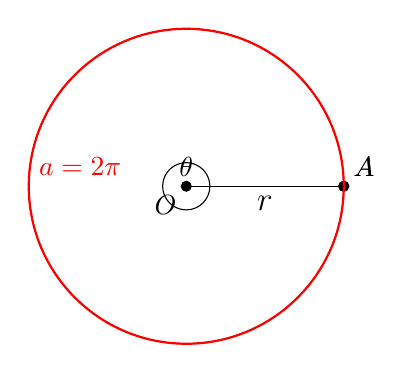
\begin{tikzpicture}
    \def\radius{2cm}
    \draw (0,0) circle (\radius);
    \draw (0,0) circle (0.3cm) node[above] {$\theta$};
    \coordinate[label=below left:$O$] (O) at (0,0);
    \coordinate[label=above right:$A$] (A) at (0:\radius);
    \coordinate[label=above right:$A$] (B) at (360:\radius);
    \foreach \point in {O, A, B}
    \fill (\point) circle (2pt);
    \draw[thick, red] (A) arc (360:0:\radius) node[midway, above right] {$a=2\pi$};
    \draw (A)--(O) node[midway, below, font=\large] {$r$};
\end{tikzpicture}

\subsubsection{Radian-Degree Conversion}
\begin{align*}
&\text{Radian} \longrightarrow \text{Degree} \left(\frac{\pi}{180^{\circ}}\right)\\
&\text{Radian} \longleftarrow \text{Degree} \left(\frac{180^{\circ}}{\pi}\right)
\end{align*}

\newpage
\subsection{Trig Ratios and Special Angles}
The triangles found in a geometry set are a $45^{\circ}-45^{\circ}-90^{\circ}$ triangle and a $30^{\circ}-60^{\circ}-90^{\circ}$ triangle. These triangles can be used to construct similar triangles with 
the same special relationships among the sides.

\begin{figure}[ht]
    \centering
    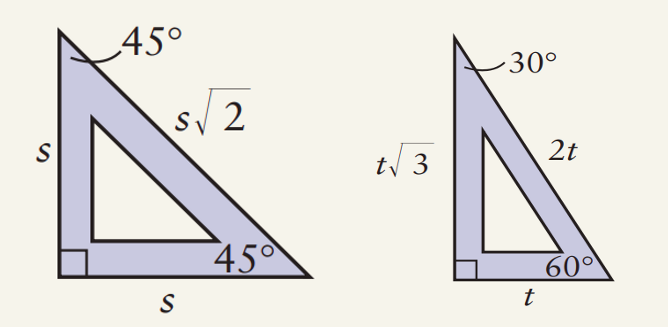
\includegraphics[width=0.5\textwidth]{imgs/special trigs.PNG}
\end{figure}

\begin{align*}
&\sin \left(\frac{2 \pi}{3}\right) = \frac{\sqrt{3}}{2}, \quad &
&\csc \left(\frac{2 \pi}{3}\right) = \frac{2}{\sqrt{3}}, \\
&\cos \left(\frac{2 \pi}{3}\right) = -\frac{1}{2}, \quad &
&\sec \left(\frac{2 \pi}{3}\right) = -2, \\
&\tan \left(\frac{2 \pi}{3}\right) = -\sqrt{3}, \quad &
&\cot \left(\frac{2 \pi}{3}\right) = -\frac{1}{\sqrt{3}}
\end{align*}


\begin{table}[htbp]
\centering
\caption{Special Angles and Trigonometric Ratios}
\label{tab:special_angles}
\begin{tabular}{|c|c|c|c|c|c|c|c|}
\hline
Angle & Degrees & Radians & \( \sin \theta \) & \( \cos \theta \) & \( \tan \theta \) & \( \csc \theta \) & \( \sec \theta \) \\ \hline
\( 0^\circ \) & \( 0^\circ \) & \( 0 \) & \( 0 \) & \( 1 \) & \( 0 \) & undefined & \( 1 \) \\ \hline
\( 30^\circ \) & \( 30^\circ \) & \( \frac{\pi}{6} \) & \( \frac{1}{2} \) & \( \frac{\sqrt{3}}{2} \) & \( \frac{1}{\sqrt{3}} \) & \( 2 \) & \( \frac{2}{\sqrt{3}} \) \\ \hline
\( 45^\circ \) & \( 45^\circ \) & \( \frac{\pi}{4} \) & \( \frac{\sqrt{2}}{2} \) & \( \frac{\sqrt{2}}{2} \) & \( 1 \) & \( \sqrt{2} \) & \( \sqrt{2} \) \\ \hline
\( 60^\circ \) & \( 60^\circ \) & \( \frac{\pi}{3} \) & \( \frac{\sqrt{3}}{2} \) & \( \frac{1}{2} \) & \( \sqrt{3} \) & \( \frac{2}{\sqrt{3}} \) & \( 2 \) \\ \hline
\( 90^\circ \) & \( 90^\circ \) & \( \frac{\pi}{2} \) & \( 1 \) & \( 0 \) & undefined & \( 1 \) & undefined \\ \hline
\end{tabular}
\end{table}
\subsubsection*{Example}
Determine exact values of the six trigonometric ratios for an angle of $\frac{3 \pi}{4}$
\begin{align*}
&\sin \left(\frac{3\pi}{4}\right) = \frac{\sqrt{2}}{2}, \quad \csc \left(\frac{3\pi}{4}\right) = \sqrt{2}, \\
&\cos \left(\frac{3\pi}{4}\right) = -\frac{\sqrt{2}}{2}, \quad \sec \left(\frac{3\pi}{4}\right) = -\sqrt{2}, \\
&\tan \left(\frac{3\pi}{4}\right) = -1, \quad \cot \left(\frac{3\pi}{4}\right) = -1.
\end{align*}

You can use the unit circle and special triangles to determine exact values for the trigonometric ratios of the special angles $0, \frac{\pi}{6}, \frac{\pi }{4}, \frac{\pi }{3}$ and $\frac{ \pi}{2}$

\newpage
\section*{Unit Circle }
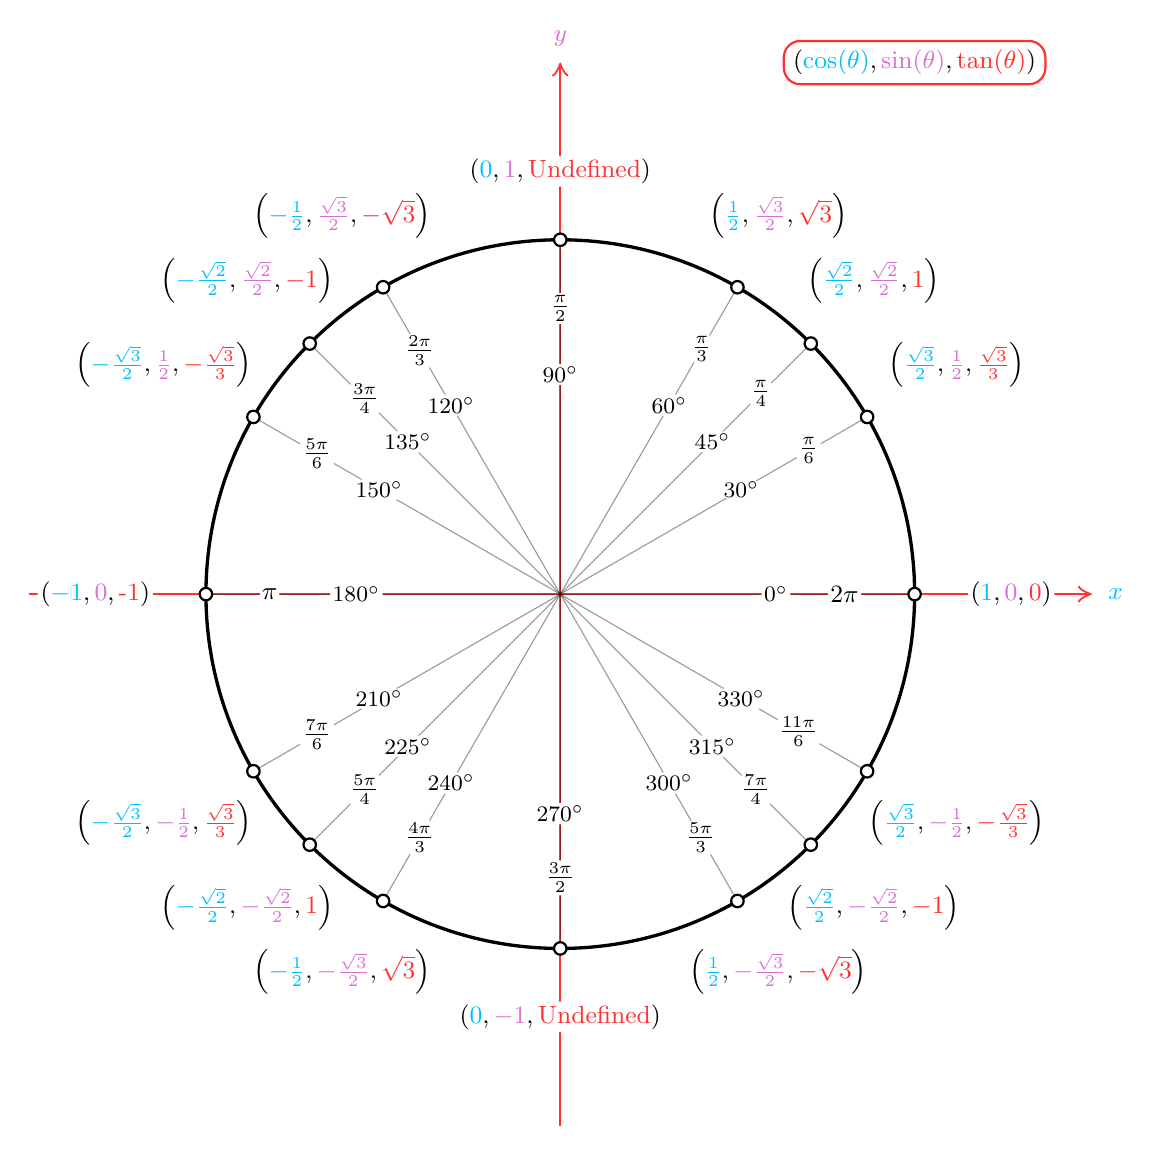
\begin{tikzpicture}[scale=4.5, font=\small]
    \definecolor{r}{HTML}{ff3030}
    \definecolor{b}{HTML}{00bfff}
    \definecolor{o}{HTML}{DA70D6}
    \def\angles{
        0/2\pi/1/0/0,
        30/\frac{\pi}{6}/\frac{\sqrt{3}}{2}/\frac{1}{2}/\frac{\sqrt{3}}{3},
        45/\frac{\pi}{4}/\frac{\sqrt{2}}{2}/\frac{\sqrt{2}}{2}/1,
        60/\frac{\pi}{3}/\frac{1}{2}/\frac{\sqrt{3}}{2}/\sqrt{3},
        90/\frac{\pi}{2}/0/1/\text{Undefined},
        120/\frac{2\pi}{3}/-\frac{1}{2}/\frac{\sqrt{3}}{2}/-\sqrt{3},
        135/\frac{3\pi}{4}/-\frac{\sqrt{2}}{2}/\frac{\sqrt{2}}{2}/-1,
        150/\frac{5\pi}{6}/-\frac{\sqrt{3}}{2}/\frac{1}{2}/-\frac{\sqrt{3}}{3},
        180/\pi/-1/0/\text{-1},
        210/\frac{7\pi}{6}/-\frac{\sqrt{3}}{2}/-\frac{1}{2}/\frac{\sqrt{3}}{3},
        225/\frac{5\pi}{4}/-\frac{\sqrt{2}}{2}/-\frac{\sqrt{2}}{2}/1,
        240/\frac{4\pi}{3}/-\frac{1}{2}/-\frac{\sqrt{3}}{2}/\sqrt{3},
        270/\frac{3\pi}{2}/0/-1/\text{Undefined},
        300/\frac{5\pi}{3}/\frac{1}{2}/-\frac{\sqrt{3}}{2}/-\sqrt{3},
        315/\frac{7\pi}{4}/\frac{\sqrt{2}}{2}/-\frac{\sqrt{2}}{2}/-1,
        330/\frac{11\pi}{6}/\frac{\sqrt{3}}{2}/-\frac{1}{2}/-\frac{\sqrt{3}}{3}
    }
    \begin{scope}[every node/.style={inner sep=1pt, outer sep=0pt}]
        \foreach \a/\at/\x/\y/\t in \angles {
            \begin{pgfinterruptboundingbox}
                \node (x) at (\a : 1.15) [anchor=\a-180] {\phantom{$\textstyle\left({\color{b} \x}, {\color{o} \y}, {\color{r} \t}\right)$}};
                \clip [rounded corners] (x.south west) rectangle (x.north east) (-1.6, -1.6) -- (1.6, -1.6) -- (1.6, 1.6) -- (-1.6, 1.6) -- cycle;
                \node (x) at (\a : 0.85) [anchor=\a] {\phantom{$\textstyle\at$}};
                \clip [rounded corners] (x.south west) rectangle (x.north east) (-1.6, -1.6) -- (1.6, -1.6) -- (1.6, 1.6) -- (-1.6, 1.6) -- cycle;
                \node (x) at (\a : 0.65) [anchor=\a, font=\footnotesize] {\phantom{$\textstyle\a^\circ$}};
                \clip [rounded corners] (x.south west) rectangle (x.north east) (-1.6, -1.6) -- (1.6, -1.6) -- (1.6, 1.6) -- (-1.6, 1.6) -- cycle;
                \clip (\a : 1) circle [radius=.5pt] (-1.6, -1.6) -- (-1.6, 1.6) -- (1.6, 1.6) -- (1.6, -1.6) -- cycle;
            \end{pgfinterruptboundingbox}
        }

        \draw [r, thick] (-1.5, 0) edge [-{Classical TikZ Rightarrow[length=5pt, width=6pt]}] (1.5, 0) node at (1.5, 0) [right=5pt] {$\textstyle\color{b} x$}
        (0, -1.5) edge [-{Classical TikZ Rightarrow[length=5pt, width=6pt]}] (0, 1.5) node at (0, 1.5) [above=5pt] {$\textstyle\color{o} y$};
        \draw [very thick] (0, 0) circle [radius=1];

        \foreach \a/\at/\x/\y/\t in \angles { \draw [opacity=.4] (0, 0) -- (\a : 1); }
    \end{scope}

    \scoped [every node/.style={inner sep=1pt, outer sep=0pt}] {
        \foreach \a/\at/\x/\y/\t in \angles {
            \node at (\a : 1.15) [anchor=\a-180, rounded corners] {$\textstyle\left({\color{b} \x}, {\color{o} \y}, {\color{r} \t}\right)$};
            \node at (\a : 0.85) [anchor=\a, rounded corners] {$\textstyle\at$};
            \node at (\a : 0.65) [anchor=\a, rounded corners, font=\footnotesize] {$\textstyle\a^\circ$};
            \draw [thick] (\a : 1) circle [radius=.5pt];
        }
    }

    \node at (1, 1.5) [thick, draw=r, rounded corners=6pt] {$\textstyle\left({\color{b} \cos(\theta)}, {\color{o} \sin(\theta)}, {\color{r} \tan(\theta)}\right)$};
\end{tikzpicture}
\newpage 

\subsection{Equivalent Trigonometric Expression}
\textbf{Definition: Equivalent Trigonometric Expressions}

Equivalent trigonometric expressions refer to different algebraic representations of the same trigonometric function or identity. Two trigonometric expressions are considered equivalent if they produce the same value for all possible inputs (angles).

For example, consider the Pythagorean identity:
\[
\sin^2(x) + \cos^2(x) = 1
\]
This equation demonstrates that the sum of the squares of the sine and cosine of an angle \( x \) is always equal to 1. Thus, the expressions \( \sin^2(x) + \cos^2(x) \) and \( 1 \) are equivalent.

Similarly, expressions such as \( \tan(x) \) and \( \frac{\sin(x)}{\cos(x)} \) are equivalent, as they represent the same trigonometric function, tangent.

Understanding equivalent trigonometric expressions is crucial for simplifying complex trigonometric equations, identities, and functions, as well as for solving trigonometric equations efficiently.

\begin{figure}[ht]
    \centering
    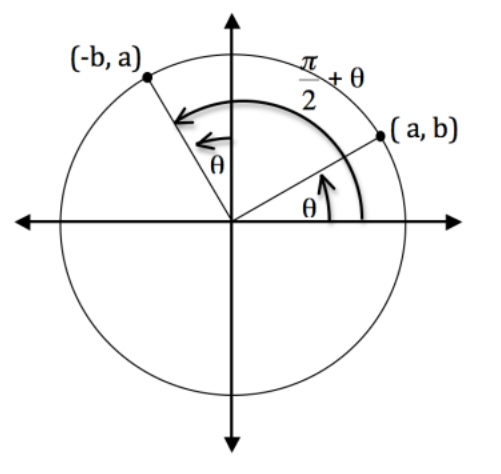
\includegraphics[width=0.5\textwidth]{imgs/circle equivalent.PNG}
\end{figure}
\begin{center}
\centering
$$
\begin{array}{|c|c|c|c|}
\hline \sin \left(\frac{\pi}{2}+\theta\right)=\cos \theta & \csc \left(\frac{\pi}{2}+\theta\right)=\sec \theta & \sin \left(\frac{\pi}{2}-\theta\right)=\cos \theta & \csc \left(\frac{\pi}{2}-\theta\right)=\sec \theta \\
\hline \cos \left(\frac{\pi}{2}+\theta\right)=-\sin \theta & \sec \left(\frac{\pi}{2}+\theta\right)=-\csc \theta & \cos \left(\frac{\pi}{2}-\theta\right)=\sin \theta & \sec \left(\frac{\pi}{2}-\theta\right)=\csc \theta \\
\hline \tan \left(\frac{\pi}{2}+\theta\right)=-\cot \theta & \cot \left(\frac{\pi}{2}+\theta\right)=-\tan \theta & \tan \left(\frac{\pi}{2}-\theta\right)=\cot \theta & \cot \left(\frac{\pi}{2}-\theta\right)=\tan \theta \\
\hline
\end{array}
$$
\end{center}

\subsection{Compound Angle Formulas}

The compound angle formulas are as follows:
\begin{align*}
& \sin(x+y)=\sin x \cos y+\cos x \sin y\\
& \sin (x-y)=\sin x\cos y-\cos-\cos x \sin y\\
& \cos(x+y)=\cos x\cos y -\sin x \sin y\\
&\cos (x-y)=\cos x \cos y+\sin x \sin y
\end{align*}
\subsubsection{Proof: }
\begin{figure}[ht]
    \centering
    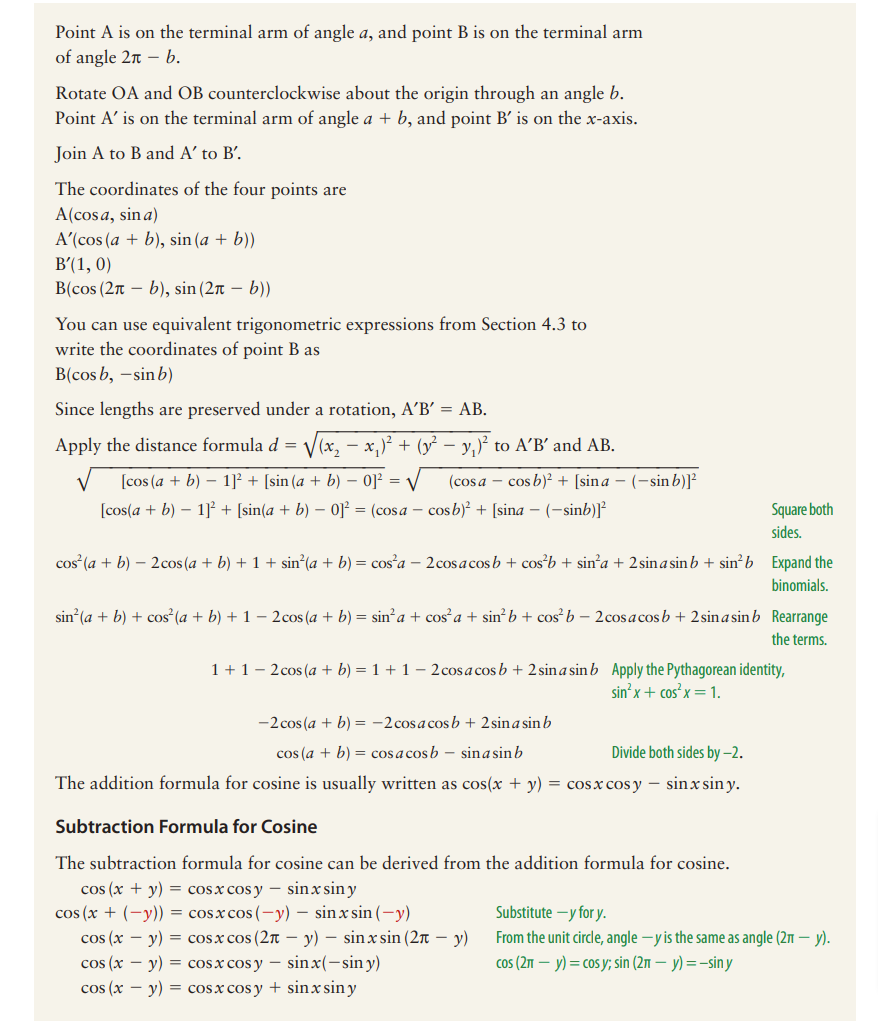
\includegraphics[width=0.9\textwidth]{imgs/proof.png}
\end{figure}

\subsubsection{Addition Formula for Sine}
Recall the cofunction identities $\sin x=\cos \left(\frac{\pi}{2}-x\right)$ and $\cos x=\sin \left(\frac{\pi}{2}-x\right)$.
Apply these and the subtraction formula for cosine.
$$
\begin{aligned}
\sin (x+y) & =\cos \left[\frac{\pi}{2}-(x+y)\right] \quad \text{Apply a cofunction identity.}\\
& =\cos \left[\left(\frac{\pi}{2}-x\right)-y\right] \quad \text{Regroup the terms in the argument.}\\
& =\cos \left(\frac{\pi}{2}-x\right) \cos y+\sin \left(\frac{\pi}{2}-x\right) \sin y \quad \text{Apply the subtraction formula for cosine.}\\
& =\sin x \cos y+\cos x \sin y \quad \text{Apply cofunction identities.}
\end{aligned}
$$
\subsubsection{Subtraction Formula for Sine}
The subtraction formula for sine can be derived from the addition formula for sine, following the approach used for the subtraction formula for cosine.
$$
\begin{aligned}
& \sin (x+(-y))=\sin x \cos (-y)+\cos x \sin (-y) \quad \text { Substitute }-y \text { for } y \\
& \sin (x-y)=\sin x \cos y+\cos x(-\sin y) \\
& \sin (x-y)=\sin x \cos y-\cos x \sin y
\end{aligned}
$$

\subsubsection*{Example}
The angles $\alpha$ and $\theta$ are located in the FIRST quadrant. If $\sin\theta=\frac{2}{3}$ and $\sin \alpha=\frac{1}{2}$, find $\cos(\theta, \alpha)$

\subsubsection*{Solution}
\begin{align*}
    \cos(\theta- \alpha)&=\cos \theta \cos \alpha+\sin \thet  \sin \alpha\\
\end{align*}
We are told that these are first quarter  so that we know the signs of all the trig ratios using CAST rule. Other than that we can use right angle to find all other trig ratios for the two angles
\begin{align*}
    &=\left(\frac{\sqrt{5}}{3}\right)\left(\frac{\sqrt{3}}{2}\right)+\left(\frac{2}{3}\right)\left(\frac{1}{2}\right)\\
    &=\frac{\sqrt{15}}{6}+\frac{2}{6}\\
    &=\frac{\sqrt{15}+2}{6}
\end{align*}
\newpage

\subsection{Prove Trig Identities }


    \textit{Quotient Identity :} $\tan \theta=\frac{\sin \theta}{\cos \theta}$

\textit{Pythagorean Identity:} $\sin ^2 \theta+\cos ^2 \theta=1$ (from the unit circle)

\textit{Reciprocal Identities :}
$$
\begin{array}{ll}
\csc \theta=\frac{1}{\sin \theta} ; \quad \sin \theta=\frac{1}{\csc \theta} \\
\sec \theta=\frac{1}{\cos \theta} ; \quad \cos \theta=\frac{1}{\sec \theta} \\
\tan \theta=\frac{1}{\cot \theta} ; \quad \cot \theta=\frac{1}{\tan \theta}
\end{array}
$$

\textit{Compound Angle Formulas:}
$$
\begin{aligned}
\sin (x+y) & =\sin x \cos y+\cos x \sin y \\
\sin (x-y) & =\sin x \cos y-\cos x \sin y \\
\cos (x+y) & =\cos x \cos y-\sin x \sin y \\
\cos (x-y) & =\cos x \cos y+\sin x \sin y
\end{aligned}
$$
\textbf{Reciprocal of Trigonometry}
  \begin{spreadlines}{1.5ex}
    \begin{alignat*}{2}
      \csc(x) & = \tfrac 1 {\sin(x)}, \quad & \tan(x) & = \tfrac {\sin(x)} {\cos(x)} \\
      \sec(x) & = \tfrac 1 {\cos(x)}, \quad & \cot(x) & = \tfrac {\cos(x)} {\sin(x)}
    \end{alignat*}
  \end{spreadlines}
\subsection{Applying the Basic Identities}
When you prove trig identities, you are trying to do anything you can with the known trig identities in order to transform the two sides and make them look like each other.\\


You may need to work on BOTH sides of the equal sign, but start first with the side that looks the most complicated. Generally you want to take complicated and make it look more simple.\\


It is important the a for each step along the way, you state what identity or math operation you have used.

\subsubsection{Exercises}  
\begin{enumerate}
    \item[a)] Prove $\frac{1+\tan x}{1+\cot x}-\frac{1-\tan x}{\cot x-1}$ 
    \item[b)] Prove $\csc 2x+\cot 2x=\cot x$ 
\end{enumerate}
\end{document}